\section{Durchführung}
\label{sec:Durchführung}

Das homogene $\vec{B_0}$ wird durch Einlassung der Proben in einen Permanentmagneten 
realisiert. Senkrecht dazu erzeugt die Modulationsspule zusätzlich ein Wechselfeld im Probenbereich,
durch welches eine Probenmagnetisierung induziert. Die präzendierende Magnetisierung
bewirkt zudem einen Induktionsstrom in der Spule, der als Nachweis für die Magnetisierung fungiert.
Weiterhin ist die Spule zusammen mit einem Kondensator variabler Kapazität Teil eines Schwingkreises
mit einer korrespondierend zur Lamorfrequenz abstimmbaren Resonanzfrequenz.

Ein in Abbildung \ref{fig:aufbau} schematisch dargestelltes NMR-Spektrometer dient zur weiteren
Analyse des Induktionsstroms.

\begin{figure}
    \centering
    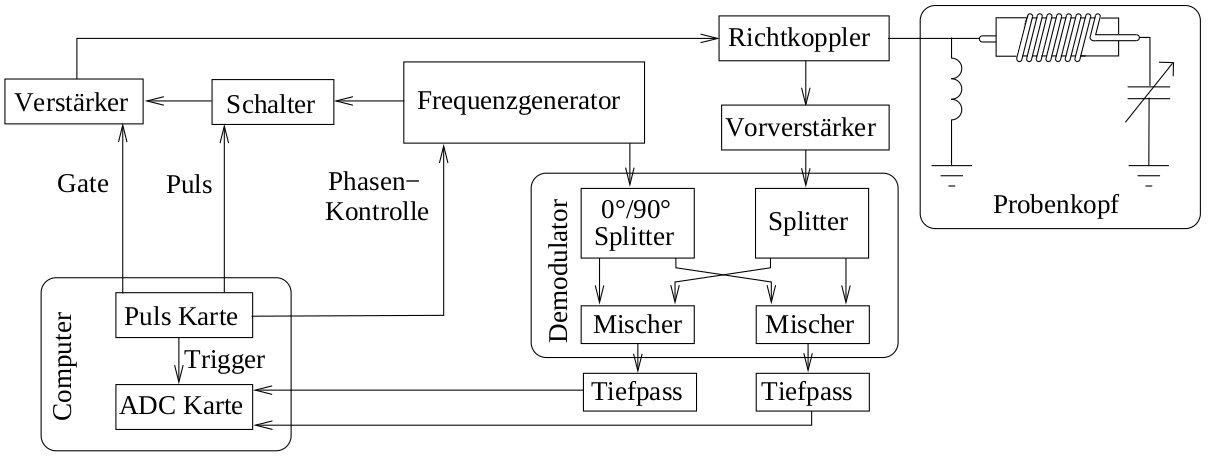
\includegraphics[scale=0.4]{content/aufbau.png}
    \caption{Aufbau und Blockschaltbild eines NMR-Spektrometers \cite{Anleitung2}.}
    \label{fig:aufbau}
\end{figure}

Der eingebaute Richtkoppler trennt Ein- und Ausgangssignale voneinander.
Die eingeheden Pulse werden durch verstärkte gemischte Signale eines Computers und Frequenzgenerators erzeugt.
Detektiert wird das Signal des Induktionsstroms nach Vorverstärkung nach dem Prinzip der Quadraturdetektion.
Dazu wird es mit einem phasenverschobenem Signal des Frequenzgenerators gemischt und schließlich von einem
Oszilloskop dargestellt.

Vor Messbeginn ist eine Justage der Versuchsapparatur mit einer Kupfersulfatlösungsprobe notwendig.
Durch einen Puls auf die Spule wird ein FID erzeugt, dessen Schwingungen durch Einstellung der Resonanzfrequenz
reduziert werden sollen. Eine Phaseneinstellung lässt das Signal in einem der Detektionskanäle
nahezu verschwinden.
Zudem wird ein optimaler Feldgradient über die sogeannten Shims eingestellt, sodass die 
Feldhomogenität maximiert wird.
Dann wird die $\SI{180}{\degree}$-Pulslänge und somit die doppelte $\SI{90}{\degree}$-Pulslänge
durch Minimierung des FID ermittelt.
Es wird eine große Periodendauer von $P = \SI{0.5}{\second}$ übergeben, die dafür sorgt,
dass die Magnetisierung vor dem folgenden Puls relaxiert.

Zur Untersuchung einer Wasserprobe wird dessen $T_1$ über eine $\SI{180}{\degree}$-$\SI{90}{\degree}$-Pulsfolge
mit $P = \SI{10}{\second}$ gemessen. Dies erfolgt durch Variation dieser Zeit zwischen den Pulsen
und der Amplitudenmessung des FID.

Zur $T_2$-Bestimmung werden ein $\SI{90}{\degree}$-Puls gefolgt von vielen $\SI{180}{\degree}$-Pulsen.
Die Signalbildwerte werden vom Oszilloskop gespeichert.

Zur Diffusionsmessung wird eine $\SI{90}{\degree}$-$\SI{180}{\degree}$-Pulsfolge angewandt
und die z-Komponente des Feldgradients wird umgepolt und dann maximal eingestellt.
Die gemessenen Spin-Echos werden dann am Oszilloskop bezüglich ihrer Signalhöhe und Lage im Zeitintervall 
zwischen den Pulsen analysiert

Weiterhin wird aufrund der Temperaturabhängigkeit der Homogenität des $B_0$ die sich ggf. 
ändernde Temperatur $T$ vor und nach den Messungen mit einem Thermoelement ermittelt.
